\section{Prototyping the device}
\label{Chap:Prototype}
We need to connect the parts previously mentioned correctly so that they can communicate with each other.
Most electronic components are accompanied by a datasheet created by its manufacturer
which details the behavior of the component,
its electrical and non-electrical characteristics,
its physical design,
pin layout,
and a typical application circuit.
This typical application circuit allows us to connect the component in the way intended by its manufacturer.
An example of this application circuit is a clipping shown in figure \ref{Fig:MPUAppCircuit} from the datasheet \cite{Datasheet:MPU6000} for the MPU-6000.
\begin{figure}
\begin{center}
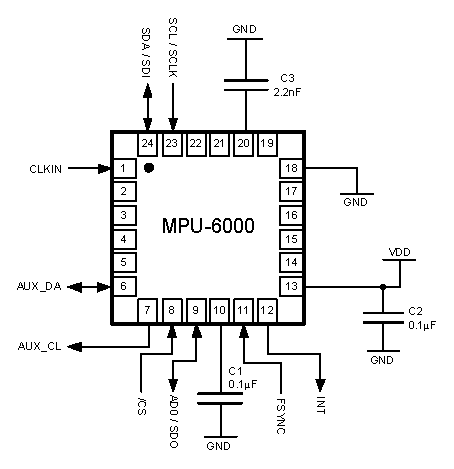
\includegraphics{images/MPU600OpCircuit.eps}
\caption{Typical operating circuit for the MPU-6000}
\label{Fig:MPUAppCircuit}
\end{center}
\end{figure}
As we can see,
the typical application circuit for the sensor shows us the pin layout of the chip,
along with any external components that need to be connected.
In this case, it shows three capacitors that must be connected to the chip.
Similar to the MPU-6000,
all the components we have selected for our device design have their respective datasheets which contain information on how they should be operated.
Using these datasheets,
a master circuit was created for our device.
This circuit was designed in the EAGLE PCB Design software.

\subsection{Overview}
\label{Sec:PCBDesign}
All components in the final device are connected to each other using a printed circuit board.
A PCB replaces wires between components by copper traces on the board,
which are lines made of copper, so that electricity is conducted across them.
Creating a PCB requires three steps, the first being circuit design.
Once the circuit is designed, the components are laid out on a PCB, and traces are created based on the circuit design.
The third process comprises of using this layout to create the actual PCB.
This third step is completed by a PCB manufacturer after we provide them with our PCB layout design.
The benefit of creating a schematic in EAGLE instead of directly creating a layout connected by traces
is that the software uses the connections in the schematic to guide us while connecting the pins or pads of the different components.
This reduces the chances of an incorrect connection between two components,
reducing any mistakes that might creep into our final PCB design and cost us money as we re-manufacture our PCB.
\begin{figure}
\begin{center}
\includegraphics[width=0.8\textwidth]{images/EagleScreen.jpg}
\caption{Screenshot of EAGLE PCB's schematic editor.}
\label{Fig:EaglePCBScreen}
\end{center}
\end{figure}

\subsection{Unit testing}
\label{Sec:UnitTesting}
We need to test each component separately and make sure they work as expected.
Although most parts have a low failure rate,
it is easier to work through with our devices knowing where a bug is 
if one shows up.
Unit testing is a method of testing individual units of source code to check if they work as expected before introducing them into a larger piece of code.
We extend this to our device creation process by testing each unit of hardware separately.
We would have to test the microcontroller, the sensor, the memory chip, the USB to UART bridge and the battery charger separately.
The microcontroller would have to be the first component to be tested because the other components require a master device that controls them.

\subsubsection{Micrcontroller testing}
To test the microcontroller we used a simple ``Hello World'' program.
Since microcontrollers do not have a display, instead of displaying text,
it is easier to just blink an LED using one of the pins.
Pseudo code to blink the LED is show in in listing \ref{LST:LEDHello}.
We programmed our microcontroller using IAR's Code Composer Studio,
and then flashed the microcontroller using the software and the MSP430 Flash Emulation Tool.
If our connections were correct,
the LED would turn on for one second,
then turn off for another second.
This cycle would repeat indefinitely, creating the illusion of a light blinking slowly.

\lstset{
  language=C,
  aboveskip=3mm,
  belowskip=3mm,
  showstringspaces=false,
  columns=flexible,
  basicstyle={\small\ttfamily},
  numbers=none,
  numberstyle=\tiny\color{black},
  keywordstyle=\color{black},
  commentstyle=\color{black},
  stringstyle=\color{black},
  breaklines=false,
  breakatwhitespace=true,
  tabsize=3,
frame=b
}

\begin{lstlisting}[caption=Program to blink LED.,label=LST:LEDHello]
/* We want to blink forever */
while(1)
{
	/* Create a delay. Our clock is at 32768 Hz */
	__delay_cycles(32768);
	FlipLEDStatus();  
}
\end{lstlisting}

\subsubsection{Sensor testing}
\label{Sec:SensorTesting}
\begin{figure}
\begin{center}
\includegraphics[width=0.6\textwidth]{images/CAT6MPU.jpg}
\caption{Photo of a MPU6000 breakout board connected to a CAT5 cable}
\label{Fig:CAt5MPU}
\end{center}
\end{figure}

After confirming that the microcontorller chip is performing as expected,
we tested our sensor. Breakout boards were previously discussed in section \ref{Sec:Breakouts},
which allow us to prototype sensors without worrying about soldering them.
Breakout boards for the MPU-6000 were obtained from an Ebay seller.
The breakout board has 6 pins that need to be connected for operation,
which means we need 6 wires between the microcontroller and the breakout board.
These pins on the breakout board were connected to the microcontroller target board using a CAT5 cable as can be seen in figure \ref{Fig:CAt5MPU}.
This is the same cable used for Ethernet connections, and thus was easy to obtain.
As shown in the same figure,
a regular CAT5 cable consists of 4 pairs of twisted wires,
so one pair in this cable was not needed.
This pair was connected to the GND pin on the microcontroller to reduce noise.

The MPU6000 uses SPI for communication.
The datasheet mentions that once the sensor is powered on and awake,
the sensor will start recording what the acceleration and angular velocity are.
This information is stored in an internal memory on the sensor which can be read using SPI instructions.
We initially had trouble verifying if our sensor is working correctly and did not know if the sensor was faulty,
or if there was a mistake in our connections or code.
The datasheet for the sensor mentions a register called ``WHO\_AM\_I'' which contains he device's I$^2$C address.
This address by default is set to 0x68.
Since this register contains constant data, we can read it to check if the device is indeed correctly connected.

After some troubleshooting we learned that the length of the cable was too long for SPI communication and the signal would lose strength.
Also, SPI is time sensitive, so if the cable length was too long,
the delay created between two times would be too high,
causing incorrect data to be received.
We fixed this by reducing how long the cable was.
In the final design the length the signal would have to travel would be very small since the chips would be laid out next to each other,
so this was not an issue we needed to worry about.
Once it was established that the sensors were working correctly and SPI communication between them was also as expected,
we carried out simple tests where the acceleration on one axis would turn an LED on if positive,
otherwise turn it off.
Since gravity would show as -1 g on the Z Axis in the earth frame of reference,
we could test all three sensor axes by rotating the sensor and observing the LED's behavior.
These tests concluded that communication between the sensor and microcontroller was as expected.

\subsubsection{Memory chip testing}
\label{Sec:MemoryTesting}
Our memory chip was tested to check if SPI communication was up and running.
As seen in Section \ref{Sec:Memory},
we created our own breakout board to break the pins out from the memory chip.
The datasheet for our memory chip mentions a command known as ``Manufacturer and Device ID''.
Issuing this command to the memory chip requests the memory chip to send 4 bytes of data to the master device.
These bytes identify the device and contain other information about it. 
For example, the second byte contains the family code and the density code,
telling us what the size of the memory is.
We only need the first byte, which is 0x1F.
Once we connected our memory chip to the microcontroller we sent this command from the master to the slave,
and received 0x1F.
This confirmed that we had connected the memory chip correctly.

Our next step was to store data from the sensor into the memory.
Since both the devices use the SPI bus,
it was possible to connect the devices to the same pins on the microcontroller.
Before reading sensor values or storing them,
we check if the device ID's are received correctly.
This was done every time the microcontroller booted up.
On our initial attempt, the memory chip did not respond with the correct device ID.
This meant that even if we were sending correct data,
it was not being received correctly with the new connection.
After some testing we realized that this was because the cable to the sensor was too long for SPI,
and timing errors were being created.
Once we reduced the length of this cable,
data transfer behaved as expected,
and we were able to record data from the sensor,
then flush it to the memory.

\subsection{Circuit design}
\label{Sec:CircuitDesign}

\begin{figure}
\begin{center}
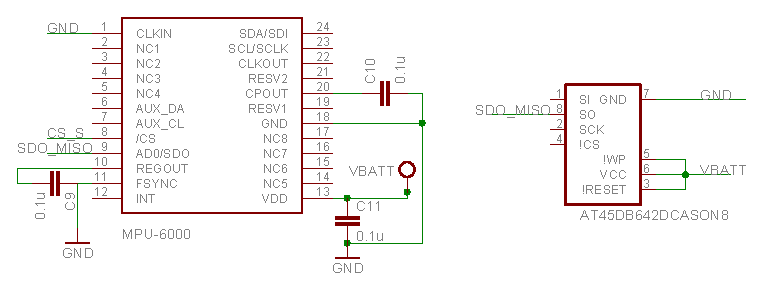
\includegraphics[width=0.8\textwidth]{images/MPU6000Circuit.eps}
\caption{Circuits designed for the MPU 6000 (left) and the AT45DB642D (right).}
\label{Fig:MPUCkt}
\end{center}
\end{figure}

\begin{figure}
\begin{center}
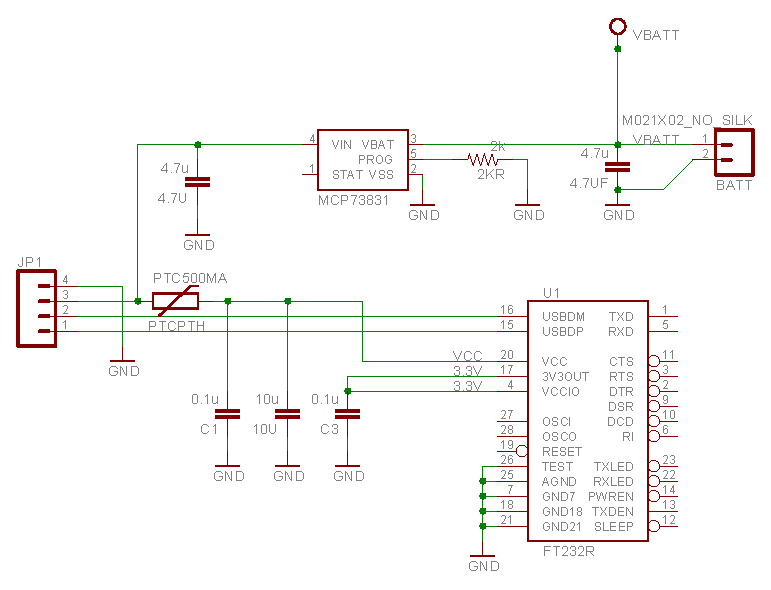
\includegraphics[width=0.8\textwidth]{images/USBPOWER.eps}
\caption{Circuits designed to power the circuit and connect the USB to UART bridge.}
\label{Fig:USBPOWER}
\end{center}
\end{figure}

\begin{figure}
\begin{center}
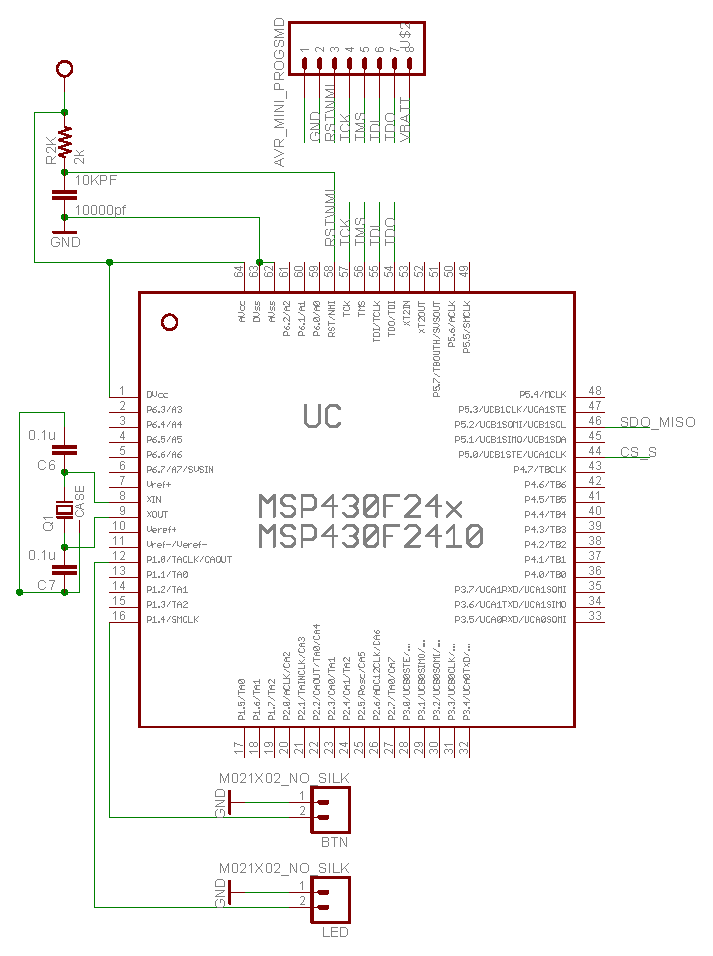
\includegraphics[width=0.8\textwidth]{images/MSP430CKT.eps}
\caption{Circuits designed to operate the MSP430F248.}
\label{Fig:MSP430CKT}
\end{center}
\end{figure}

\begin{figure}
\begin{center}
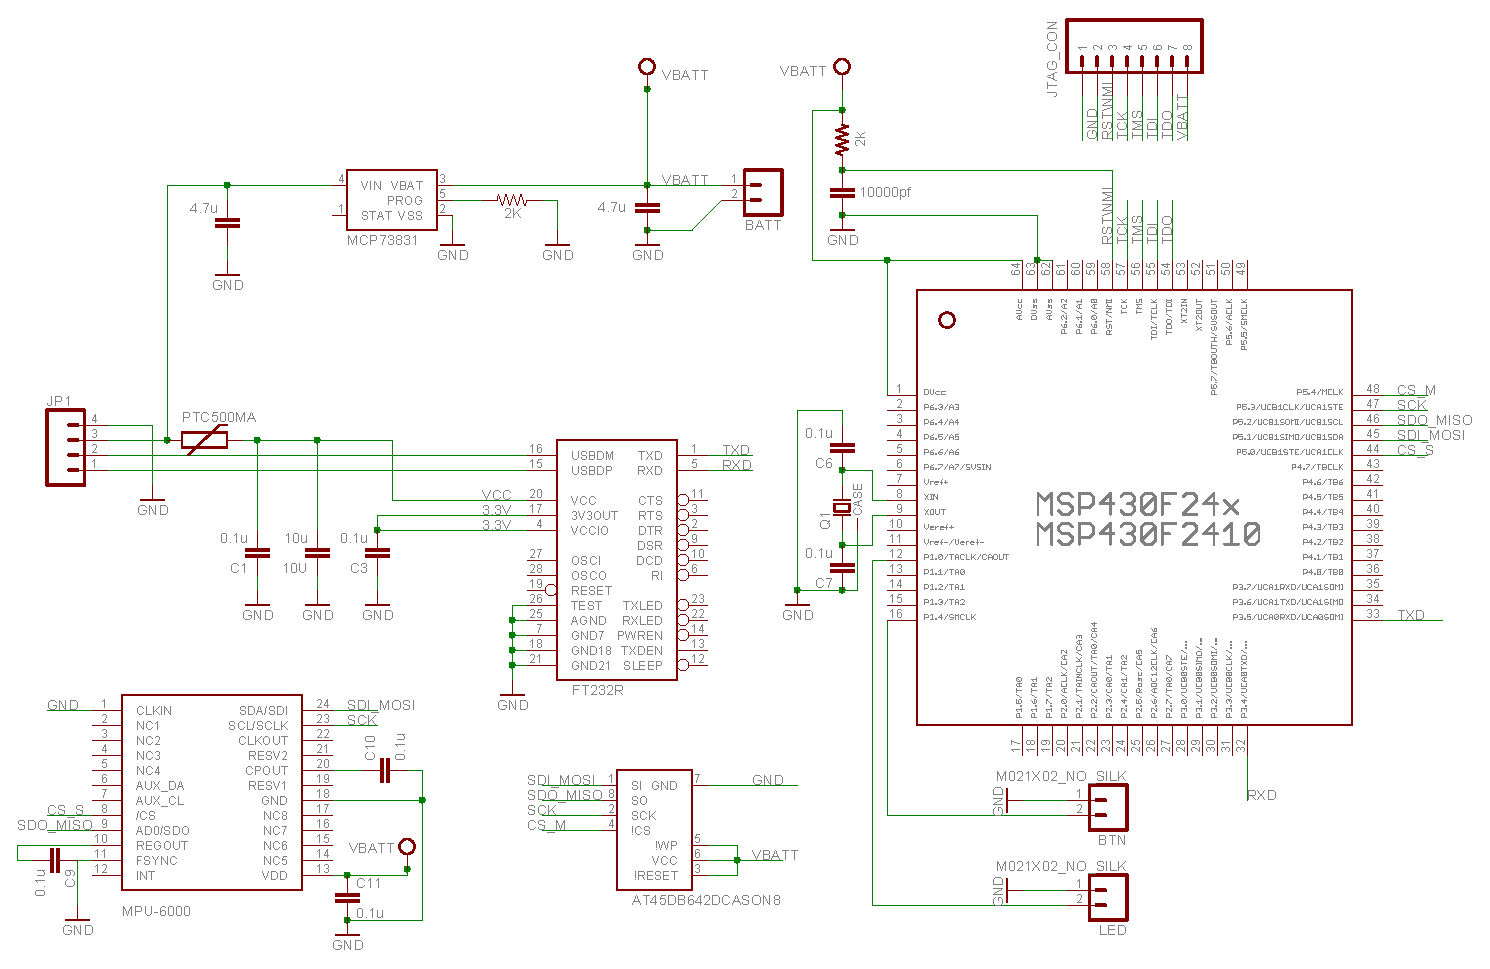
\includegraphics[angle=-90,width=0.8\textwidth]{images/FULLCKT.eps}
\caption{The complete circuit for the wrist motion activity tracker.}
\label{COMPCKT}
\end{center}
\end{figure}
The circuits for different parts of the device that we designed are shown in figures \ref{Fig:MPUCkt}, \ref{Fig:USBPOWER}, and \ref{Fig:MSP430CKT}.
The complete circuit we designed after consulting the different datasheets is shown in figure \ref{COMPCKT}.
This circuit was created using EAGLE PCB's schematic layout tool.
Each component had its circuit created separately,
and later these circuits were connected together to create the final device.
A screenshot of Eagle PCB's schematic editor is shown in figure \ref{Fig:EaglePCBScreen}.
We used a breadboard to prototype the device once we had a circuit design available.
The breadboard allowed us to connect our components together and program the microcontroller with a reduced amount of soldering, 
and this can be seen in figure \ref{Fig:BreadBoardProto}.

\begin{figure}
\begin{center}
\includegraphics[width=0.8\textwidth]{images/BreadProto.jpg}
\caption{Photograph of prototype made using a breadboard. Not shown: USB cable for connection.}
\label{Fig:BreadBoardProto}
\end{center}
\end{figure}


\subsection{Programming and testing}
\label{Sec:Programming}
With our components connected,
it was possible to program our microcontroller and make it perform the required functions.
Our program polls the sensors repeatedly.
The data from these sensors is then stored in the microcontrollers memory until the total data crossed a threshold.
Once this threshold was crossed, the data would be sent to the memory chip.
A simplified version of the microcontroller code is seen in figure \ref{Fig:MainAlgo}.
\begin{figure}
\begin{center}
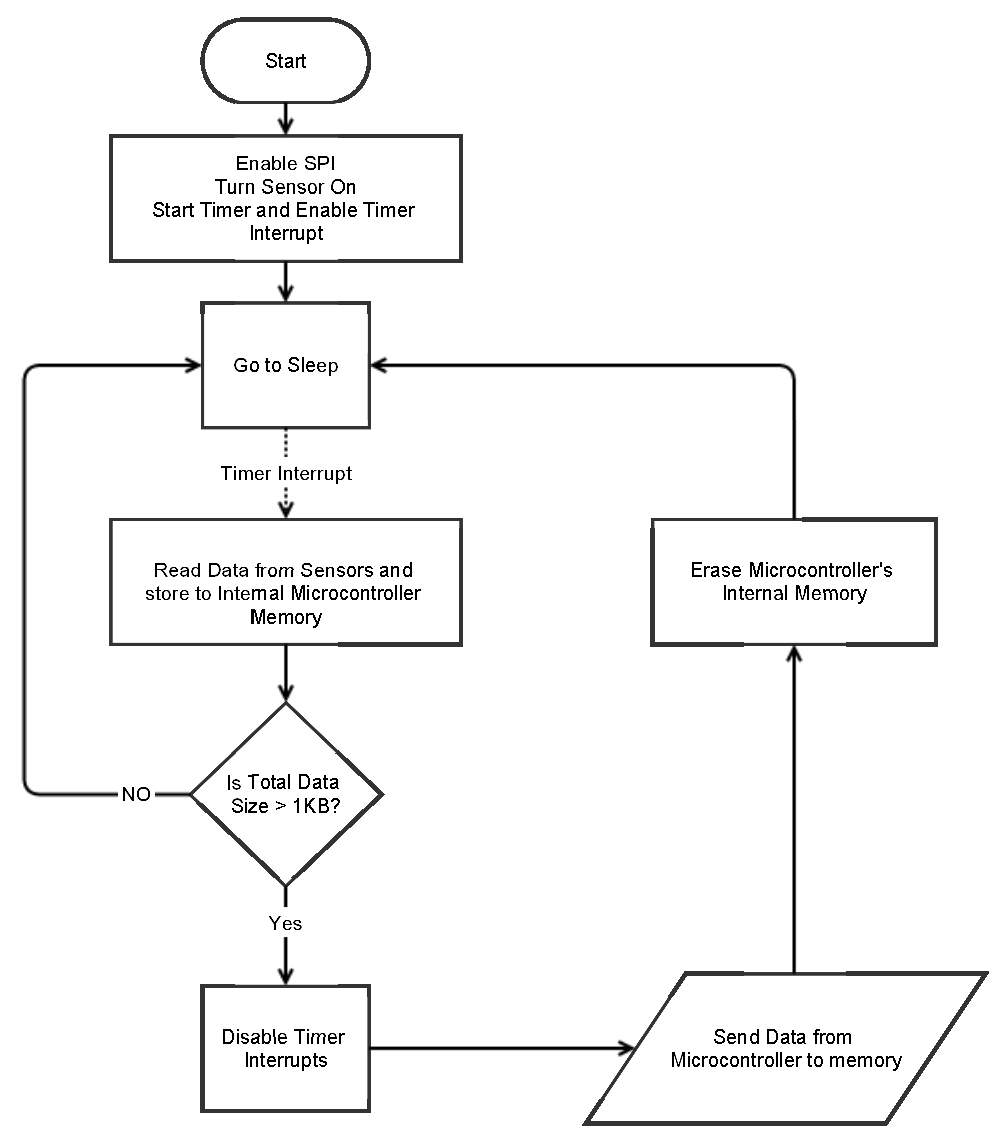
\includegraphics[width=0.8\textwidth]{images/MainAlgo.eps}
\caption{Flowchart showing simplified algorithm used for the device.}
\label{Fig:MainAlgo}
\end{center}
\end{figure}
To test the battery life of our device,
a video stream was setup which had a camera pointed at the device.
We connected a multimeter measuring voltage to the battery,
and had its display visible in the frame.
The video stream also had a time stamp to show how the battery voltage dropped as the device operated.
Since the device would blink an LED every 11.33 seconds,
it was easy to monitor the device operation through this video.
When the device stopped operating,
the LED would stop blinking.
We could watch the video to see the exact time when this happened,
and have an accurate idea on the battery life of our device.
These experiments were repeated three times each for the 90mAh and 130mAh Turnigy Nano-tech batteries.

\subsubsection{PCB layout}
The PCB was laid out using EAGLE PCB's layout editor based on our tested circuit design.
The software first generates parts and their footprints from the schematic we created.
This can be seen in figure \ref{Fig:Layout1}.
The parts are placed in randomized locations by the software.
The software connects these parts by direction lines (seen in yellow in figure \ref{Fig:Layout1}) called signals.
We sized the PCB to be smaller than the case so that it would fit easily, and moved the parts around so that pins that need to connect components are close to each other.
This can be see in figure \ref{Fig:Layout2}.
The signals were routed through the copper board,
using the signals as a guide, and this process is shown in figure \ref{Fig:Layout3}.
This process is like a puzzle where we are trying to draw lines through objects that we cannot cross.
Seven revisions were required for our final PCB.
\begin{figure}
\begin{center}
\includegraphics[width=0.8\textwidth]{images/Layout1.jpg}
\caption{Screenshot of Eagle PCB's layout editor.}
\label{Fig:Layout1}
\end{center}
\end{figure}
\begin{figure}
\begin{center}
\includegraphics[width=0.7\textwidth]{images/Layout2.jpg}
\caption{Parts to be routed after placing on the PCB in EAGLE PCB software.}
\label{Fig:Layout2}
\end{center}
\end{figure}
\begin{figure}
\begin{center}
\includegraphics[width=0.7\textwidth]{images/Layout3.jpg}
\caption{Routing in EAGLE PCB. The incomplete (thick) red line is guided by the (thin) yellow signal line.}
\label{Fig:Layout3}
\end{center}
\end{figure}
\subsubsection{PCB manufacture}
PCBs were manufactured by OSH Park\footnote{http://oshpark.com}.
Most PCB manufactures expect a high volume of production (100 - 1000 PCBs per order).
We only required a few prototype PCBs so our order was only a few PCBs.
OSH Park takes multiple orders from its clients and combines this into a large PCB.
This is then cut into the requested PCBs and sent back to the client.
This process takes time, but costs less than what most other PCB manufacturers charge.
For example,
Advanced Circuits LLC,
a well known PCB manufacturer charges \$120 for 4 bare bones PCBs,
and has a turnaround time of a week.
These PCB lack any kind of silkscreen,
or printed text,
which means it is hard to know where parts are located,
or what their value is.
Since there is no silkscreen,
the copper traces on the PCB oxidize over time and lose conductivity.
OSH Park,
on the other hand offers high quality PCBs at a lower cost.
The turn around time is much longer (approximately 21 days),
however we were able to procure 6 PCBs for a total of \$15,
costing us approximately \$2.5 per PCB.

To create our PCBs, we uploaded our PCB layout file generated by Eagle PCB to the OSH Park website.
The website shows you an approximate render of how the PCB will look once it is delivered,
and also notifies you if it thinks there could be issues with part placement (for example, parts may be too close to the border).

\subsubsection{Software}
\label{Sec:Software}
Work done by Concha \cite{concha2014study} shows PhoneView,
a tool developed to analyze data collected by an iPhone.
Instead of the wrist based activity monitor that we are developing,
work done by the group previously used an iPhone mounted on the wrist.
This data could be loaded into PhoneView,
which would then plot the instantaneous values of each sensor versus time,
allowing us to process this data as signals.
PhoneView would accept data that was stored in ASCII.
This means that each sensor reading would require three digits,
each requiring 1 byte.
Raw data that was 8 MB in size would expand to 24 MB if stored as ASCII.
We modified the source code of PhoneView to allow for our data from the wrist motion activity tracker.

\subsubsection{Soldering}
\label{Sec:Soldering}
\begin{figure}
\begin{center}
\includegraphics[width=0.5\textwidth]{images/BarePCB.jpg}
\caption{The bare PCB received after fabrication.}
\label{Fig:PCBBare}
\end{center}
\end{figure}
A photograph of the bare PCB can be seen in figure \ref{Fig:PCBBare}.
As can be seen,
most components are going to be surface mounted to this PCB,
and there are very few through hole components.
Throughout this thesis we have emphasized on how small the components we are dealing with are.
These components are so small that we lost a couple of the parts when trying to handle them because someone was breathing too hard.
In the industry,
pick and place machines are used to move these components around.
Solder is first applied to all the pads.
These machines then use vacuum to pick up the delicate components,
and cameras to inspect them. 
Once the components are placed on a PCB,
the PCB is sent to an oven where the solder melts,
and the components are soldered once it cools down.
We did not have access to an industrial facility with these features,
so we would have to use a different technique to solder these components.
Our first attempt was mentioned when we discussed our memory chip in section \ref{Sec:Memory}.
As seen, we flipped the chip over to expose its pads,
then soldered thin strands of a multi strand wire to the chip.
These strands connected to thicker wire at the other end,
which allowed us to use the chip as a through hole component.
All this was done very carefully under a microscope.
The MPU-6000 integrated chip has pads that are much smaller than what our memory chip did.
It was not feasible to solder strands to this chip because of the same reason,
so we researched for other techniques.

\subsubsection{Z axis conductive tape}
\label{Sec:ZTape}
Sparkfun.com demoed a new product from 3M,
called the Z-Axis Tape,
just as we were looking for methods to solder our sensor \cite{Web:SFETAPEV}.
The Z-Axis Conductive Tape is described by Sparkfun as ``an easy to use,
pressure sensitive double sided tape designed for connecting,
bonding and grounding flex circuits and PCBs.''
In theory, we should be able to place this tape between the PCB and our integrated chip,
and have conductivity between the pad on the PCB and those on the chip.
The datasheet for this conductive tape mentions that it is filled with small conductive particles which allow it to conduct electricity through its thickness,
however these particles are spaced far enough to maintain electrical insulation.
The datasheet also mentions that the minimum distance between two adjacent conductors should be 0.4 mm or greater to ensure electrical insulation,
however, the method used to bond the parts together and temperature would affect this number.
The MPU-6000 datasheet mentions a pitch of 0.25 mm between two pads,
which was smaller than the suggested distance of isolation by the tape.
However given that the tape was expected to operate under extreme conditions of temperature (-40$\degree$ C-70$\degree$C),
we decided to try this tape to bond our sensor chip to the PCB.
Our experiment showed that sufficient conductivity was attained after 24 hours to allow SPI communication between the sensor and the microcontroller,
however this conductivity was lost over time,
within seven days in our case.

This process concluded that the Z-Axis tape was not a permanent alternative solution to soldering the sensor to our PCB.

\subsubsection{Reflow Skillet}
\label{Sec:ToasterReflow}
As an incentive to its clients,
Sparkfun offers tutorials on multiple topics,
and has a tutorial on different soldering methods \cite{Web:SparkfunSoldering}.
This tutorial mentions four different methods that a hobbyist electrical engineer can use to prototype a device based on SMT components:

\begin{description}

	\item[Hand Soldering] \hfill \\
	This is the regular method of soldering with a soldering iron that we have already tried with our memory chip.
	\item[Toasting] \hfill \\
	This process involves placing solder paste and parts on the PCB,
	then heating them in a temperature regulated toaster oven to the temperature required by the solder to melt.
	This melts the solder, and when cooled provides us with a PCB with components connected.
	We did not have access to a toaster with an accurate temperature control,
	and so could not test this method.
	\item[Industrial Ovens] \hfill \\
	Similar to the method mentioned above,
	this technique uses industrial ovens specially constructed for SMD soldering.
	We did not have access to these industrial ovens.
	\item[Hot Air Rework] \hfill \\
	This method uses a hot air blower that increases the temperature of the PCB to that of the solder melting point.
	This method is used frequently to desolder or rework SMT components.
	We tried this method,
	but did not get a high degree of success.
	One of the reasons for failure was that our parts would fly away under the air pressure,
	and it was not feasible to hold down the part in place correctly because our hands would shake while doing so.
	\item[Hot Plate Reflowing] \hfill \\
	This method requires that pads on the PCB have solder paste applied to them.
	Once this is done,
	we place the components over their approximate locations on the PCB.
	After this is done,
	we place the PCB with the components over a skillet that is heated to the temperature of the solder.
	If everything goes right,
	the molten solder will behave like a liquid,
	and due to force of adhesion,
	parts will align themselves correctly in place.
\end{description}
\hfill \\
\begin{figure}
\begin{center}
\includegraphics[width=0.5\textwidth]{images/stencil.jpg}
\caption{Photograph of the stencil used to apply solder paste to the PCB.}
\label{Fig:Stencil}
\end{center}
\end{figure}
Based on the different techniques mentioned above,
we used the hot plate reflowing method.
Similar to OSH Park, a website, OSH Stencils accepts EAGLE PCB layout files,
and provides laser cut stencils for the PCB.
This stencil was used to apply solder paste only to the exposed pads of the PCB.
A photo of the stencil is shown in figure \ref{Fig:Stencil}.
We placed some components: the microcontroller, memory chip,
sensor and the USB to UART chip on the PCB by hand.
This was done because it was very hard to place the smaller components
like capacitors and resistors by hand and not have them move other parts in the process.
After about 23 seconds on the skillet,
we could see the solder melt and the parts fall into place.
Through hole components and smaller components like the crystal oscillator and resistors were individually soldered later by hand under a microscope.
Figure \ref{Fig:PCBMicro} shows the hand soldering process through the microscope's lens. The Final PCB can be seen in figure \ref{Fig:PCBwithCase}.
\begin{figure}
\begin{center}
\includegraphics[width=0.95\textwidth]{images/PCBMicro.jpg}
\caption{Photograph showing crystal oscillator being soldered under a microscope.}
\label{Fig:PCBMicro}
\end{center}
\end{figure}
\begin{figure}
\begin{center}
\includegraphics[width=0.95\textwidth]{images/PCBBare.jpg}
\caption{Photograph the PCB after soldering, along with top side of case.}
\label{Fig:PCBwithCase}
\end{center}
\end{figure}


\subsubsection{Final device}
\label{Sec:FinalDevice}
We programmed the microcontroller with the same code used in our breadboard based prototype.
The case was modified to seat the LED and the button,
with the LED and the button stuck to the upper side of the case using hot glue.
The PCB was placed under this button, and the battery was the last part to enter the case.
The case had a ring which allowed a wrist watch style strap to fit through,
and we added this to the case.

\subsection{Verification of logged data}
\label{Sec:Motion Data}
Now that our device was ready to be worn on the wrist,
we performed some experiments to verify that it works as expected.
Our aim for this device was to create a wrist motion activity tracker that would track wrist movements all day,
and also be comfortable when worn for extended intervals.
We would have to test the comfort of the device,
and also verify that the data it was reporting was correct.
To check if the data being reported was correct,
we setup an experiment where the user would wear both the wrist motion activity tracker,
and the iPhone from the PhoneView experiment performed by our group earlier.
The user would then make characteristic movements which could be identified easily by looking at the signals in PhoneView or WristView.